\documentclass{article}
\usepackage{amsmath}
\usepackage{amssymb}
\usepackage[utf8]{inputenc}
\usepackage{soul}
\usepackage{graphicx}

\usepackage{color}
\definecolor{orange}{RGB}{255,127,0}

\graphicspath{{img/}}
\setlength{\parindent}{0pt}


\begin{document}
	\title{CW 16/17 Summary}
	\author{Alexander Pastor}
	\date{23.04.2017}
	\maketitle
	\tableofcontents
	\newpage
	
	\section{Wireless Network Fundamentals}
	
	\subsection{Why Wireless?}
	
	Wireless networks have a number of potential advantages over wired networks.
	
	\medskip
	
	These include mobility hence flexibility, ease of deployment, potential cost reduction.
	
	\smallskip
	
	Disadvantages include exposition to malevolent intrusion and at times lower speed. 
	
	\subsection{Basic Terminology}
	
	\vskip 0.1in
	
	A (802.11) network consits of \emph{stations, the wireless medium, access points and the distribution system}.
	
	\bigskip
	
	\emph{stations} 
	
	Defining aspect: devices used for data transfer among them. Devices with wireless interfaces, mostly, but not limited to handheld devices or laptops.
	
	\bigskip
	
	\emph{wireless medium} 
	
	In our case two radio frequency layers (2.4 GHz and 5GHz).
	
	\bigskip
	
	\emph{access points} 
	
	The points through which stations can access the network. Their main purpose is acting as a wireless-to-wired bridge, i.e. translating wireless frames to wired frames to communicate with the rest of the world.
	
	\bigskip
	
	\emph{distribution system}
	
	The logical network component that forwards (possibly "translated") frames from the access points to their destination. 802.11 does not specify a technology, but Ethernet is dominant. 
	
	From this fact one can derive that wireless technology is not meant to be a substitute for wired technology, but as a supplement to provide more mobility to users.
	
	\bigskip
	
	There are different two different basic types of networks, which gives rise to the next set of terminology.
	
	\bigskip
	
	\emph{basic service set (BSS)} 
	
	A basic service set is the basic unit of a wireless network and simply comprises of a set of communicating computers. The covered area is called basic service area. These basic service sets come in two flavors. One is independent basic service set (IBSS), the other is infrastructure basic set service. Infrastructure basic service sets include access points, while independent basic service sets have no access points.
	
	\medskip 
	
	This means IBSSs have no connection to the outer world, hence the name "independent". Useful for short-ranged, short-lived ad-hoc networks for the purpose of data exchange during a conference. 
	
	\bigskip
	
	\emph{service set identifier (SSID)}
	
	Serves as a name for the service set.
	
	\bigskip
	
	\emph{extended service set (ESS)}
	
	Created by linking several BSSs together with a backbone network. All linked sets share the same SSID, thus are not distinguishable from the viewpoint of the user.
	
	\bigskip
	
	\emph{virtual access points}

	Multiple virtual access points on the same physical access point make it possible to have several virtual ESSs with only one set of physical hardware. Particularly useful if you want to have networks with different levels of security or want to restrict access to certain resources.
	
	\bigskip
	
	\emph{atomic operation}
	
	Set of operations that is individable, i.e. if one operation out of the set fails the whole atomic operation fails.
		
	\bigskip
	
	\emph{fragment}
	
	Large (management or higher-layer) frames would sometimes exceed a certain maximum length. If that would happen they are instead split into several smaller fragments. The point is this way they are less susceptible to interference, because the likelihood of an atomic operation succeeds increases. This may increase throughput. However, this comes at a price of additional management and frame overhead. 
	
	\bigskip
	
	\section{WLAN, LTE-U and LAA}
	
	To make network devices beautifully compatible industrial standards are needed. This is what the following section will discuss.
		
	\subsection{802 and 802.11}
	
	The following is a picture of the IEEE 802 norm family. 802 deals with \emph{local area networks} (LANs) and \emph{metropolitan area networks} (MANs). The specified protocols reside in the physical and data link layer. 802.11 is about \emph{wireless LAN} (WLAN). As of now only the working groups of 802.1 (higher layer LAN protocols), 802.3 (Ethernet) and 802.11 are active.
	
	\begin{figure}[h] \label{802-tree}
		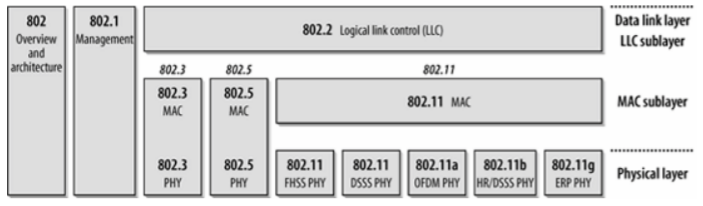
\includegraphics[width=\textwidth]{802-tree}
	\end{figure} 
	
	A way of defining network technology is to define the services it provides, much like defining an API for software.
	
	\bigskip
	
	802.11 provides the following: distribution, integration, association, reassociation, disassociation, authentication, deauthentication, confidentiality, MAC SDU (MSDU) delivery, Transmit Power Control (TPC), Dynamic Frequency Selection (DFS).
	
	\smallskip
	
	A detailed description is omitted.
	
	\bigskip
	
	\textbf{Note:} It is worth to mention that while 802.11 supports seamless BSS transition within an ESS, it does not support seamless ESS transition, as higher layer connections are interrupted.
	
	\subsection{The LTE Unlicensed Family}

	LTE stands for Long-Term Evolution. It is a wireless communication standard for mobile devices. Despite not meeting the criteria defined by the ITU-R (the radio division of a specialized United Nations agency) to be labeled as 4G service it is marketed as such and has achieved an almost global presence. It is an improvement over preceding generations in terms of speed and other technical aspects such as spectral efficiency (measures transmission rate per bandwidth).
	
	\medskip
	
	\textbf{Note:} LTE Advanced has been formally acknowledged to meet 4G's criteria and is a candidate 4G technology. The other candidate is 802.16m better known as "WiMax" (\emph{Worldwide Interoperability for Microwave Access}) and is currently available in more than 150 countries.
	
	\bigskip
	
	LTE-U stands for LTE Unlicensed and is a proposal originally made by Qualcomm for the use of LTE technology in the unlicensed 5GHz band. However, the "indigenous" dual-band WiFi equipment vendors fear performance losses for their technology if LTE-U was to share a part in the band. LAA which expands to \emph{License Assisted Access} is a term used by Ericsson to describe a similar technology. LAA uses a LBT contention protocol. 
	
	\bigskip
	
	Qualcomm and their allies Verizon and Ericsson claim that LTE-U family technologies would better neighbors to WiFi in terms of joint AND individual throughput, than WiFi itself. Google and the WiFi-alliance claim WiFi performance losses of up to 40\%. Both parties mutually accuse the other's studies, tests and allegations would be profoundly biased and unfair.
	
	\subsection{MAC Challenges}
	
	Wireless transmissions based on radio waves suffer from multiple physical problems wired transmissions don't have. Overcoming these obstacles is the challenge for designers of MAC protocols.
	
	\subsubsection{Link Quality}
	
	Noise, interference and multipath fading make wireless signals less reliable both in terms of bit error rate, establishing and keeping up a connection at all, in case a node moves into a dead spot. 
	
	\medskip
	
	Radio link quality is also influencing the possible maximum data transmission rates. As signal quality degrades one has to slow down the data transmission rate to make sure a useful (correctly demodulatable) signal arrives at the other side. The overall volatile nature of wireless transmission also forces the technology to be highly adaptive in terms of for instance speed regulation. The keyword here is \emph{multirate support}.
	
	\subsubsection{The Hidden Node Problem}
	
	In Ethernet networks CSMA/CD is used to detect collisions. This is not the case for wireless networks.
	
	\bigskip
	
	Since the signal quality of every radio wave transmitter degrades over distance each station has a limited range.

	\bigskip

	Suppose node B was in range of nodes A and C, but A and C not in each other's range, then A is called hidden node from the viewpoint of C and vice versa.
	
	\bigskip
	
	Collisions from hidden nodes are hard to detect, because wireless transceivers are \emph{half-duplex}, i.e. able to transmit and receive packets, but not at the same time. The reason is that due to attenuation the magnitude of received waves can be several powers below those of the originally transmitted waves. If a node was to simultaneously send and receive the received signal would simply "drown in the sea of transmission noise". 
	
	\medskip
	
	\textbf{Note:} It is possible to receive and transmit at the same time, but this requires very intricate and thus costly signal processing hardware. 
	
	\bigskip
	
	For networks of sufficient capacity (delay-bandwidth-product) so-called \emph{Request-to-Send-Singnals} (RTS) as well as \emph{Clear-To-Send-Signals} (CTS) can aid to achieve the goal of collision avoidance. However, this palpably increases the duration of an atomic operation, which then consits of RTS, CTS, the data frame and the ACK (and interframe spacing).
	
	\bigskip
	
	\color{blue}
	[thought experiment] If I had nodes with very different power levels belonging to the same BSS (for instance let edge nodes have more "buzz" in order to cover peripheral areas). Imagine now that an arbitrary node A wants to transmit and issues a RTS. A set of nodes \{B\} in vicinity of this node will subsequently respond with a CTS and shutdown nodes in their vicinity. Suppose the CTS doesn't reach an edge node E, but the edge node's power would be big enough to interfere with the original sender. Suppose that without loss of generality range A equals the range of each member of the set {B}. This implies that E's range is more than twice as big as A's. Is this possible scenario with 802.11? The question has come up once I read that 802.11 features energy regulation to adapt the nodes' respective ranges to prevent similar scenarios to what I described. Below a little sketch to illustrate what I'm asking.
	\color{black}
	
	\begin{figure}[h] \label{signal-ranges}
		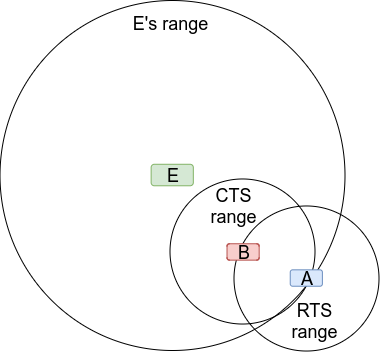
\includegraphics[height=7cm, keepaspectratio]{signal-ranges}
		\centering
	\end{figure}
	
	\bigskip
	\color{red}
	[answer] This scenario is possible, however not very likely. RTS/CTS is optional (used only in high-capacity environments with significant contention (gast, p.36)) and furthermore not designed to prevent but only reduce the risk of interference. 802.11's transmit power control (TPC) further reduces interference of stations with each other and also other wireless networks (Gast, p.26). The above sketch holds true especially if the only access point in the infrastructure BSS would be between A and B.
	\color{black}
	
	\subsection{How the MAC Stuff is Supposed to Work}
	
	First let's discuss the difference between CSMA/CD and CSMA/CA.
	
	\medskip
	
	A CSMA/CD-like protocol is used for the wired Ethernet. Since wired connections are full-duplex collisions can be detected. In case of a collision CSMA/CD shuts down transmission to minimize the damage dealt, i.e. minimize wasted transmission time (and also power). 
	
	\medskip
	
	As discussed earlier wireless transmissions are half-duplex and that is why collisions are not detected and we only try to avoid them. For this purpose we listen to the channel before we transmit (LBT) and optionally use the 802.11 RTS/CTS exchange.
	
	\medskip
	
	The LBT procedure is implemented as a so-called \emph{distributed coordination function} (DCF). In case contention-free service is required a function built on top, the so-called \emph{point coordination function} can be used. A \emph{quality of service} (QoS) compromise can be achieved with the \emph{hybrid coordination function} (HCF).
	
	\medskip
	
	\color{red}
	[confirmed] DCF is the only practically established MAC access function.
	\color{black}
	
	\subsubsection{Virtual Carrier Sensing and the Network Allocation Vector}
	
	\color{blue}
	[question] Is the following statement correct: 802.11 only uses physical carrier sensing while receiving and just before sending?
	\color{black}
	
	\bigskip
	
	\color{red}
	[answer] Yes. Note that the statement can be condensed to "802.11 only uses physical carrier sensing while receiving". This is due the fact that if a station is not sending it is receiving (alias listening).
	\color{black}
	
	\bigskip
	
	802.11 uses to type of carrier sensing functions to determine, whether the channel is busy or not. One is physical carrier sensing and the other virtual carrier sensing. If either sense finds a busy channel, the MAC layer reports a busy channel to the above layer.
	
	\bigskip
	
	Needless to mention, but still: the physical carrier sense alone is insufficient, because radio transceivers cannot transmit and receive at the same time. Hidden nodes make matters worse.
	
	\bigskip
	
	The so-called \emph{Network Allocation Vector} (NAV) is designed to solve this problem. Most 802.11 frames carry a duration field in which is filled in with the time in microseconds which a node expects to use the medium. Other stations can then count down from NAV to 0 before trying to transmit. This nifty trick is called \emph{virtual carrier sensing}.
	
	\subsubsection{Interframe Spacing}
	
	Interframe spacing is yet another measure to coordinate traffic. According to the simple logic that higher priority frames should have to wait less than lower priority frames  (in 802.11) there are four different fixed-duration interframe intervals (not a function of transmission rate, but dependent on physical layer protocol - "arbitrary" but fixed).
	
	\bigskip
	
	Important frames such as RTS/CTS and ACKs have the highest priority and the space between them is the \emph{short interframe space} (SIFS).
	
	\medskip
	
	Frames sent off "with the consent" of DCF and PCF respectively have interframe spaces of DIFS and PIFS.
	
	\medskip
	
	In case of transmission errors there also exists the \emph{extended interframe space} EIFS for retransmissions. 
	
	\bigskip
	
	\color{blue}
	[question] What is meant by the following statement: "Once a station has transmitted the first frame in a sequence, it has gained control over the channel. Any additional frames and their ACKs can be sent using the SIFS, which locks any other stations"? (p.42, Gast) Does this imply after seizing control over the channel there are no frame intervals of length DIFS anymore? This wouldn't make sense, because after a break of DIFS follows the contention-phase. I think the following statement would be more concise: "Once a station has transmitted the first FRAGMENT of a sequence (...) it sends any additional FRAGMENTS OF THAT ATOMIC SEQUENCE with an interframe (better interfragment) spacing of SIFS.
	\color{black}
	 
	\bigskip
	
	\color{red}
	[deferred] DIFS follows after each atomic sequence. Aggregation is not topical as of now and fragment is not specified enough to comprehensively answer this question.
	\color{black}
	 
	\subsection{Error Recovery and Backoff with the DCF}
	
	When an error is detected a retransmission has to take place. Upon retransmission a station's retry counter (one for each frame) is incremented. We distinguish between short and long frames and also between short and long retry counts. Frames longer than a threshold (typically the RTS frame length) are considered to be long, otherwise short.
	
	\bigskip
	
	After a certain number of retries has been reached the MAC layer discards these frames. Higher layers may issue further retransmissions though. From the point of the MAC layer these retransmissions are completely new and independent though and hence the retry counter starts at 0.
	
	\bigskip
	
	The reason for having different maximum retry counts for long and short frames is that longer frames require more buffer space. If we have a lower maximum retry count for them we can (potentially) save buffer space.
	
	\bigskip
	
	Another feature added to frames is a lifetime. When the specified limit is reached the frame is simply discarded and no attempt is made to (re)transmit any associated fragments.   
	
	\medskip
	
	\color{red}
	[confirmed] I think the point of this is to catch some fairly rare errors, such as that frame still lingering around will be discarded instead of taken for a valid frame of a later transmission.
	\color{black}
	
	\bigskip
	
	The DCF backoff works as follows: if two stations wanted to transmit a frame they would cause a "collision" in the contention phase. As a consequence, the number of coSPectrntention slots is roughly doubled (powers of 2 minus 1). In the subsequent contention phase they arbitrarily choose a slot. The station with the lowest slot number wins. This process is repeated until no slot collision occurs.
	
	\bigskip
	
	An exception in this concept is the \emph{Spectralink Voice Priority} (SVP) which allows frames carrying voice data to get the $0^{th}$ contention slot, hence prioritizes speech over other data. The reason is to bolster the QoS of VoIP services which are inherently vulnerable to any delays. To ensure stability however, retransmissions of speech are subject to contention.
	
	\subsection{Frame Format}
	
	Specific frame formats are omitted here. However, here are some questions.
	
	\bigskip
	
	\color{blue}
	[question] (Gast p.51 footnote) "802.11 specifies that stations should ignore frames that do not have the same BSSID (...)." But what about ESS-based services then? I assume the following: since ESSs have the same SSID for all their BSSs one could say that all BSSs of an ESS have the same BSSID. Wouldn't it be more concise to generally speak of ESSID in that case or simply of SSID in a general case?
	\color{black}
	
	\bigskip
	
	\color{orange}
	[clarification required] You said (B/E)SSIDs were employed to provide a human-readable way of distinguishing between networks. You also said in the protocols MAC-addresses were used to decide whether a packet is dropped. So I imagine that in each node exist some efficient data structures, possibly trees that save ESSs, BSSs and MAC-addresses. Is that about correct?
	\color{black}
	
	\bigskip
	
	\color{blue}
	[question] (Gast p.53) "(...) There is no higher-level protocol tag in the 802.11 frame to distinguish between higher-layer protocol types. Higher-layer protocol types are tagged with a type field by an additional header (...)." What is a tag and how are they used? If a tag is something like a higher-layer header, doesn't the second contradict the first one then?
	\color{black}
	
	\bigskip
	
	\color{orange}
	[clarification required] This still doesn't make sense to me. Could you define tag in this context?
	\color{black}
	
	\bigskip

	\color{blue}
	[question] (Gast p.53) "802.11 does not have negative ACKs for frames that fail the frame check sequence". Why not? Would this add, too much to the device complexity? 
	\color{black}
	
	\bigskip
	
	\color{red}
	[answer] Since there are no "Go-Back-N-like" accumulative ACKs negative ACKs would not provide any additional information as missing positive ACKs can be interpreted as NAKs. The reason that there are no accumulative ACKs is the half-duplex nature of wireless transmission. ACKs could be lost in the sending process.
	Furthermore, for larger N other nodes could suffer from huge delays.
	\color{black}
	
	\section{Getting to Know GNU Companion}
	
	I have built some simple block diagrams. Looking at more of this is the next top priority. A more detailed description is omitted in this summary for the sake of saving some time. More will follow in later write-ups.

	\section{Python}
	
	I bought a book and did some basic tasks. Not much more to say here, except that I'll put more effort into that during the next weeks. 
	
	\section{\LaTeX}
	
	I currently use TeX Live and TeXStudio as IDE. I have not faced any significant problems as of now.
	
	\bigskip
	
	I looked at basic functionality such as creating a title page, a structure, equation, align and other environments. Furthermore I looked at how to add pictures and text and to format these including virtual and horizontal spacing, floats, coloring, adding a text-style and more.
	
	\bigskip
	
	More features I need to look at: Generating a well-formatted table of contents, footnotes, bibliography, means to creates sketches and more.
	
	\bigskip
	
	I also acquired a \LaTeX-reference book by Helmut Kopka.
	
	
\end{document}